\documentclass{article}


% if you need to pass options to natbib, use, e.g.:
%     \PassOptionsToPackage{numbers, compress}{natbib}
% before loading neurips_2023


% ready for submission
%\usepackage{neurips_2023}
\usepackage[final]{neurips_2023}

% to compile a preprint version, e.g., for submission to arXiv, add add the
% [preprint] option:
%     \usepackage[preprint]{neurips_2023}


% to compile a camera-ready version, add the [final] option, e.g.:
%     \usepackage[final]{neurips_2023}


% to avoid loading the natbib package, add option nonatbib:
%    \usepackage[nonatbib]{neurips_2023}


\usepackage[utf8]{inputenc} % allow utf-8 input
\usepackage[T1]{fontenc}    % use 8-bit T1 fonts
\usepackage{hyperref}       % hyperlinks
\usepackage{url}            % simple URL typesetting
\usepackage{booktabs}       % professional-quality tables
\usepackage{amsfonts}       % blackboard math symbols
\usepackage{nicefrac}       % compact symbols for 1/2, etc.
\usepackage{microtype}      % microtypography
\usepackage{xcolor}         % colors
\usepackage{graphicx}

\title{Advancing PPI Prediction with ESMC-derived Embeddings}


% The \author macro works with any number of authors. There are two commands
% used to separate the names and addresses of multiple authors: \And and \AND.
%
% Using \And between authors leaves it to LaTeX to determine where to break the
% lines. Using \AND forces a line break at that point. So, if LaTeX puts 3 of 4
% authors names on the first line, and the last on the second line, try using
% \AND instead of \And before the third author name.



\author{
	Anrui Wang \\
	2023533015 \\
	\texttt{wangar2023@shanghaitech.edu.cn}\\
	\And
	Jiawen Dai \\
	2023533132 \\
	\texttt{daijw2023@shanghaitech.edu.cn}\\
	 \AND
	 Yiting Qi \\
	 2023533043 \\
	 \texttt{qiyt2023@shanghaitech.edu.cn}\\
}


\begin{document}
	
	
	\maketitle
	
	
	\begin{abstract}
		Predicting protein-protein interactions (PPIs) is crucial for understanding cellular function and disease, yet computational methods face persistent challenges in accuracy and generalizability. This work investigates how advanced protein representations from the ESM-family of large language models can enhance PPI prediction capabilities. We introduce a comprehensive pipeline that extracts high-dimensional, per-residue embeddings from the ESMC model and addresses the inherent challenge of variable sequence lengths through carefully designed processing strategies. These range from straightforward pooling methods to a sophisticated Masked Autoencoder (MAE) framework that preserves critical structural information while producing fixed-length representations. The processed embeddings serve as input to a hierarchy of supervised classifiers, culminating in a specialized Deep Neural Network (DNN) that achieves state-of-the-art performance. Our results demonstrate that the synergy between evolutionarily informed embeddings and purpose-built neural architectures provides a robust foundation for advancing computational PPI discovery.
	\end{abstract}
	
	
	\section{Introduction}

	An understanding of the intricate web of PPIs is fundamental to deciphering the mechanisms of life, as these interactions orchestrate nearly all biological processes. The disruption of these critical connections is a known driver of numerous human diseases, including cancer and neurodegenerative disorders, making the comprehensive mapping of the interactome a vital pursuit for both basic science and therapeutic development~\citep{recent_advances_ppi_2023}. While experimental techniques have laid the groundwork for our current knowledge, they are often hampered by issues of throughput, labor, and significant rates of false positives and negatives. Consequently, computational methods have emerged as indispensable complements, leveraging the explosive growth in genomic data to predict interactions \emph{in silico}. These approaches, which range from models based on functional genomics to those analyzing amino acid sequences, have shown considerable success; however, a lack of standardized evaluation and persistent discrepancies between algorithms have made it difficult to compare models and have obscured the specific inference mechanisms that underpin their predictions~\citep{pitfalls_ml_ppi_2023}.

Recognizing these challenges, our work explores whether more advanced representations of proteins can elevate predictive performance and clarify the signals driving interaction. Recent breakthroughs have demonstrated that large language models trained on the vast scale of evolutionary sequence data can learn the fundamental language of protein biology, capturing complex structural and functional properties without direct supervision~\citep{evolution_language_model_2023}. Building on this progress, we present a comprehensive pipeline that harnesses ESMC model embeddings to generate rich, context-aware protein representations. Our central hypothesis posits that these sophisticated features, when integrated with carefully designed neural architectures, can provide more robust interaction signals than traditional sequence-based approaches, ultimately advancing the precision and reliability of computational PPI prediction.
	
	
	\section{Methods}

	\subsection{Protein Embedding Extraction}

	We employed the ESMC 300M model, a state-of-the-art protein language model designed to capture evolutionary patterns in protein sequences. For each input sequence, the model generates per-residue embeddings that result in matrices of shape $(L+2) \times 960$, where $L$ represents the sequence length and the additional two positions correspond to special start and end tokens. These embeddings encode both local amino acid properties and global structural context derived from extensive evolutionary training data.
	
	\subsection{Dimensionality Standardization Strategies}

	The variable-length nature of protein embeddings necessitated the development of standardization approaches that preserve critical biological information while enabling downstream classification.
	
	\paragraph{Pooling-based approaches} Standard pooling techniques, including average and max pooling along the sequence dimension, provide the most straightforward solution for dimensionality reduction. These methods compress variable-length embedding matrices into fixed-size vectors of dimension $[1, 960]$, ensuring computational efficiency at the cost of potentially important positional and structural information.

	\paragraph{Masked average pooling} To address the information loss inherent in standard pooling while properly handling sequences of varying lengths, we developed a masked pooling strategy. This approach creates boolean masks based on actual sequence lengths, ensuring that computations exclude artificial padding positions. The mathematical formulation follows: $\mathbf{emb}_{avg} = \frac{\sum_{i=1}^{L} m_i \cdot \mathbf{emb}_i}{\sum_{i=1}^{L} m_i}$, where $m_i$ represents the mask value and $\mathbf{emb}_i$ denotes the embedding at position $i$. This methodology preserves the biological integrity of protein representations by preventing dilution from padding artifacts.

	\paragraph{Masked Autoencoder framework} Recognizing the limitations of pooling-based dimensionality reduction, we constructed an MAE to create information-rich, fixed-length representations. The framework standardizes input sequences to 1502 residues through zero-padding for shorter sequences and truncation for longer ones. 
	
	Initial training attempts revealed that the model struggled with feature learning, often converging on artificial padding patterns rather than meaningful biological signals. This challenge was addressed through several methodological refinements: normalization of input features to unit variance, implementation of robust loss functions, and critically, restriction of loss computation to biologically relevant sequence regions. The refined training protocol applies a 50\% masking strategy exclusively to non-padded positions, enabling the model to learn meaningful reconstructions of protein embeddings while avoiding interference from artificial padding.

	As demonstrated in Figure~\ref{fig:mae_recon}, the MAE's reconstruction capabilities validate our methodological improvements, showing the model's ability to recover complex sequence-level features from heavily masked inputs. The close correspondence between original and reconstructed values in unmasked regions confirms the model's learning of meaningful protein representations rather than artificial padding artifacts.
	
	\begin{figure}[h]
		\centering
		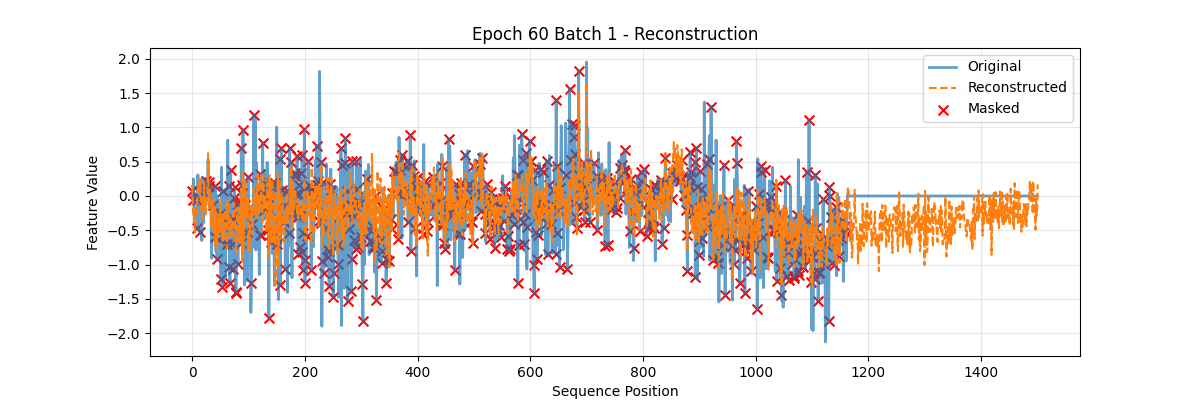
\includegraphics[width=0.7\textwidth]{imgs/epoch60_batch1.png}
		\caption{Reconstruction performance of the MAE at epoch 60. The visualization compares original embedding values (blue), reconstructed values (orange), and masked positions (red crosses). The tight alignment between original and reconstructed curves in unmasked regions demonstrates the model's capacity to learn and reproduce complex sequence-level features from incomplete data.}
		\label{fig:mae_recon}
	\end{figure}
	
	\paragraph{Feature processing strategy} An important design consideration involved the sequence of compression and concatenation operations. While joint compression of concatenated protein features could theoretically capture inter-protein dependencies, empirical evaluation revealed performance degradation with this approach. The suboptimal results likely stem from extreme length disparities between paired proteins, which create challenging training dynamics for compression models. Consequently, our final pipeline adopts individual protein compression followed by concatenation of the resulting fixed-length vectors—a strategy that consistently demonstrated superior performance.
	
	
	\subsection{Supervised Classification Framework}

	We formulated PPI prediction as a binary classification challenge, developing a progressive series of models that exploit the processed embeddings with increasing sophistication.

	\paragraph{Baseline approaches} Similarity-based methods using L2 distance and cosine similarity between protein embeddings provided initial performance benchmarks. While computationally efficient, these approaches proved insufficient for reliable interaction identification. Logistic regression offered a more principled baseline, employing learned linear combinations of joint features constructed through vector concatenation and element-wise operations to distinguish interacting from non-interacting pairs.

	\paragraph{Gradient boosting} XGBoost implementation explored non-linear modeling capabilities through ensemble methods. We evaluated five feature construction strategies: direct concatenation, element-wise addition and subtraction operations, multiplication-only features, absolute difference computation, and comprehensive combination of all approaches. Each strategy underwent feature scaling before training, with early stopping mechanisms preventing overfitting.

	\paragraph{Deep neural architecture} Our most sophisticated approach employed a specialized DNN designed to leverage the sequential nature of protein embeddings. The architecture begins with masked average pooling to handle variable-length sequences, followed by dedicated protein encoders that transform the 960-dimensional embeddings to 256-dimensional representations through linear layers, layer normalization, ReLU activation, and dropout regularization (0.3). 
	
	The encoded protein representations are concatenated and processed through an interaction prediction module comprising three fully connected layers with progressive dimensionality reduction (512 → 256 → 128 → 1). Each layer incorporates normalization, activation, and regularization components to enhance learning stability and generalization. Training employed the AdamW optimizer with OneCycle learning rate scheduling, achieving optimal convergence with a maximum learning rate of 5e-3.
	
	\section{Experiments}
    
	\subsection{Experimental Design}

	Our evaluation utilized the benchmarking gold standard dataset (benchmarkingGS v1.0), comprising 268,499 protein pairs with UniProt identifiers, interaction labels, and complete amino acid sequences. The dataset's structure facilitates comprehensive evaluation through three distinct splits: a training set of 85,329 pairs with balanced class distribution (50.00\% positive), a similarly balanced test set (Test1) containing 24,898 pairs, and a biologically realistic test set (Test2) with 136,939 pairs exhibiting natural class imbalance (9.09\% positive interactions).

	Model development and hyperparameter optimization proceeded using a validation set of 21,333 pairs (50.00\% positive) derived from the original training data. This experimental design enables assessment of both balanced classification performance and real-world generalization under realistic class distributions. AUROC served as the primary evaluation metric, providing robust comparison across different modeling approaches.

	\subsection{Performance Analysis}

	Our results demonstrate a clear progression in predictive capability with increasing model sophistication. Simple similarity metrics achieved limited effectiveness (L2 similarity: 0.5547 AUROC), while logistic regression provided substantial improvement (0.6182 AUROC). XGBoost further enhanced performance to 0.6441 AUROC through non-linear modeling capabilities.

	Our DNN architecture delivered superior results across all evaluation scenarios. On Test1, the DNN achieved 0.7283 AUROC with 65.47\% accuracy, while maintaining robust performance on the imbalanced Test2 dataset (0.7242 AUROC). The consistent performance across both test conditions validates the model's generalization capability.

	As detailed in Table~\ref{tab:results}, our approach demonstrates substantial improvements over existing sequence-based methods, achieving 7.1\% performance gains over the best reported sequence-based model (0.6800 AUROC). This advancement underscores the effectiveness of combining ESMC-derived embeddings with specialized neural architectures for computational PPI prediction.

	\begin{table}[h]
	\caption{Comparative AUROC performance across balanced and imbalanced test datasets}
	\label{tab:results}
	\centering
	\begin{tabular}{lcc}
	\toprule
	\textbf{Method} & \textbf{Test1 AUROC} & \textbf{Test2 AUROC}\\
	\midrule
	Cosine Similarity & 0.5260 & 0.5676\\
	L2 Similarity & 0.5472 & 0.5718\\
	Logistic Regression & 0.6182 & 0.6500\\
	XGBoost & 0.6638 & 0.6660\\
	\midrule
	\multicolumn{3}{c}{\textit{Literature Baseline}}\\
	\midrule
	XGBoost & 0.62 & --\\
	Sequence-based Model & 0.68 & --\\
	\midrule
	DNN (Our Method) & \textbf{0.7283} & \textbf{0.7242}\\
	\bottomrule
	\end{tabular}
	\end{table}

	\section{Conclusion}

	This investigation demonstrates that advanced protein language models can substantially enhance computational PPI prediction through the systematic integration of ESMC-derived embeddings within carefully designed classification pipelines. Our DNN architecture not only outperforms established baselines but also achieves consistent performance across both balanced and imbalanced evaluation scenarios. While the success of our framework highlights the transformative potential of combining sophisticated embeddings with purpose-built neural architectures, we recognize that predictive performance represents only one dimension of model utility in biological applications. The interpretability challenges inherent in deep learning may limit applicability where mechanistic understanding takes precedence over pure predictive accuracy, suggesting that optimal modeling approaches may vary according to specific research objectives and biological contexts.

	Looking toward future developments, more sophisticated embedding strategies could preserve greater amounts of positional and structural information currently lost during compression. Perhaps most promising is the prospect of end-to-end fine-tuning, where protein language models undergo direct optimization for interaction prediction rather than relying on fixed representations. The convergence of large-scale protein modeling with specialized prediction architectures represents a significant step forward in computational structural biology, promising increasingly powerful tools for mapping the interactome and understanding the molecular foundations underlying life's essential processes.

	\bibliographystyle{plain}
	\bibliography{references}
	
	%%%%%%%%%%%%%%%%%%%%%%%%%%%%%%%%%%%%%%%%%%%%%%%%%%%%%%%%%%%%
	
	
\end{document}